% This file was created with tikzplotlib v0.10.1.
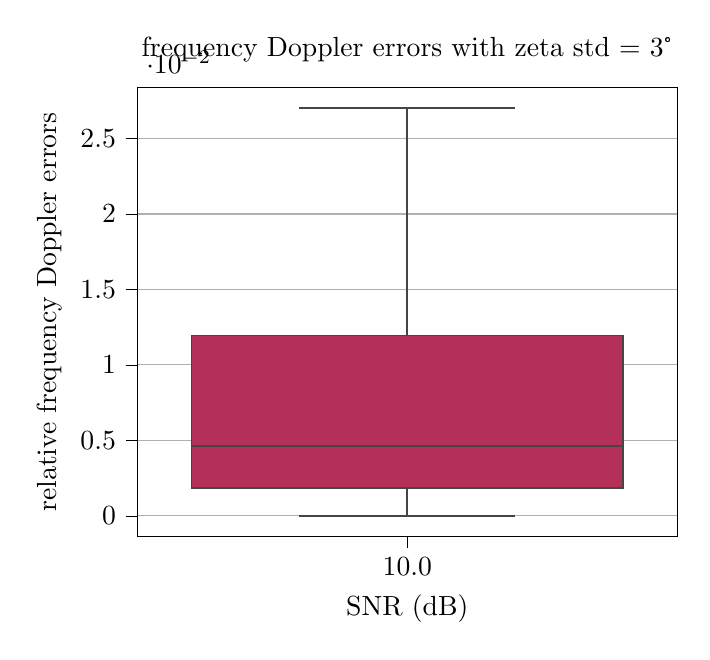
\begin{tikzpicture}

\definecolor{brown1814888}{RGB}{181,48,88}
\definecolor{darkgray176}{RGB}{176,176,176}
\definecolor{darkslategray69}{RGB}{69,69,69}

\begin{axis}[
tick align=outside,
tick pos=left,
title={frequency Doppler errors with zeta std = 3°},
x grid style={darkgray176},
xlabel={SNR (dB)},
xmin=-0.5, xmax=0.5,
xtick style={color=black},
xtick={0},
xticklabels={10.0},
y grid style={darkgray176},
ylabel={relative frequency Doppler errors},
ymajorgrids,
ymin=-0.00134890951324532, ymax=0.0283594017643156,
ytick style={color=black}
]
\path [draw=darkslategray69, fill=brown1814888, semithick]
(axis cs:-0.4,0.0018549547908983)
--(axis cs:0.4,0.0018549547908983)
--(axis cs:0.4,0.0119505623171253)
--(axis cs:-0.4,0.0119505623171253)
--(axis cs:-0.4,0.0018549547908983)
--cycle;
\addplot [semithick, darkslategray69]
table {%
0 0.0018549547908983
0 1.4682720983549e-06
};
\addplot [semithick, darkslategray69]
table {%
0 0.0119505623171253
0 0.0270090239789719
};
\addplot [semithick, darkslategray69]
table {%
-0.2 1.4682720983549e-06
0.2 1.4682720983549e-06
};
\addplot [semithick, darkslategray69]
table {%
-0.2 0.0270090239789719
0.2 0.0270090239789719
};
\addplot [semithick, darkslategray69]
table {%
-0.4 0.00461922648921448
0.4 0.00461922648921448
};
\end{axis}

\end{tikzpicture}
